\chapter{Evaluation}

The following chapter describes the evaulation and introduces the results from the testing of the prototype. 

\section{Purpose of Evaluation}



\section{Internal Test}

To test the accuracy of the prototype, an internal test were carried out. The following hypotheses has been stated for the internal test: \\\\
H\textsubscript{0}: The system works every time.\\
H\textsubscript{A}: The system does not work every time.\\\\

The test consisted of the copper plates being connected 25 times each. Firstly the index finger were tested with the thumb, secondly the middle finger. Whenever the yellow light on the system
lit up, it was considered a success. If the light did not turn on, it was considered a failure. The times it succeeded and failed were counted.\\\\

The results ended up being as follows:\\
Index finger connection test: 23 out of 25. \\
Middle finger connection test: 25 out of 25.\\\\

Another internal test has been carried out to test the accuracy of the effects. The test were conducted in a similar way, the effect were applied and then used. 
As long as the effect worked and changed the voice input, it was considered a success. \\\\

The results ended up being as follows:\\
Harmonise application effect: 18 out of 25 times. \\
Pitch shift application effect: 18 out of 25 times. \\\\

During the first tests, the system had a loose wire. The issue were fixed and the tests were then conducted once again. With the following results.\\\\

Index finger connection test: \\
Middle finger connection test: \\

\subsection{Evaluation Plan}

\subsection{Results}


\section{User Test}

\subsection{Evaluation Plan}

When conducting this user test, it is the intention to get some data from the users about the different effects and gestures. 
Initially, the users are asked to sign a consent form, see Appendix \ref{Consent} and \ref{Script} for script and consent form. They are then told to put on the glove and try to apply the effects. Afterwards, they are then asked to answer a questionnaire, see Appendix \ref{Questionnaire}. 

\subsection{Apparatus and Setup}



\begin{minipage}{\linewidth}% to keep image and caption on one page
\makebox[\linewidth]{%        to center the image
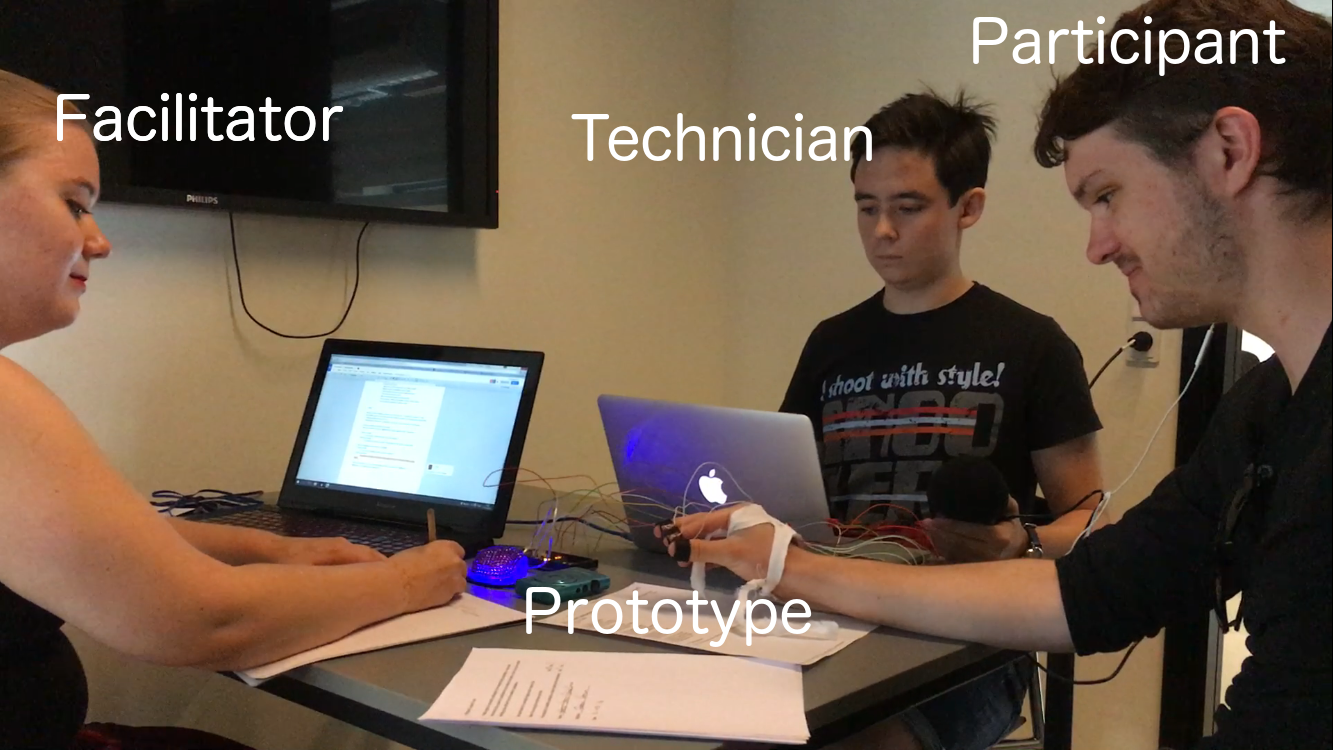
\includegraphics[keepaspectratio=true,scale=0.1]{Setup}}
\captionof{figure}{The Test Setup}\label{Setup}
\end{minipage}\\

\subsection{Results}


\section{Analysis}

\subsection{Theory}

\subsection{Results}


\section{Conclusion}